\documentclass[twoside]{book}

% Packages required by doxygen
\usepackage{fixltx2e}
\usepackage{calc}
\usepackage{doxygen}
\usepackage[export]{adjustbox} % also loads graphicx
\usepackage{graphicx}
\usepackage[utf8]{inputenc}
\usepackage{makeidx}
\usepackage{multicol}
\usepackage{multirow}
\PassOptionsToPackage{warn}{textcomp}
\usepackage{textcomp}
\usepackage[nointegrals]{wasysym}
\usepackage[table]{xcolor}

% Font selection
\usepackage[T1]{fontenc}
\usepackage[scaled=.90]{helvet}
\usepackage{courier}
\usepackage{amssymb}
\usepackage{sectsty}
\renewcommand{\familydefault}{\sfdefault}
\allsectionsfont{%
  \fontseries{bc}\selectfont%
  \color{darkgray}%
}
\renewcommand{\DoxyLabelFont}{%
  \fontseries{bc}\selectfont%
  \color{darkgray}%
}
\newcommand{\+}{\discretionary{\mbox{\scriptsize$\hookleftarrow$}}{}{}}

% Page & text layout
\usepackage{geometry}
\geometry{%
  a4paper,%
  top=2.5cm,%
  bottom=2.5cm,%
  left=2.5cm,%
  right=2.5cm%
}
\tolerance=750
\hfuzz=15pt
\hbadness=750
\setlength{\emergencystretch}{15pt}
\setlength{\parindent}{0cm}
\setlength{\parskip}{3ex plus 2ex minus 2ex}
\makeatletter
\renewcommand{\paragraph}{%
  \@startsection{paragraph}{4}{0ex}{-1.0ex}{1.0ex}{%
    \normalfont\normalsize\bfseries\SS@parafont%
  }%
}
\renewcommand{\subparagraph}{%
  \@startsection{subparagraph}{5}{0ex}{-1.0ex}{1.0ex}{%
    \normalfont\normalsize\bfseries\SS@subparafont%
  }%
}
\makeatother

% Headers & footers
\usepackage{fancyhdr}
\pagestyle{fancyplain}
\fancyhead[LE]{\fancyplain{}{\bfseries\thepage}}
\fancyhead[CE]{\fancyplain{}{}}
\fancyhead[RE]{\fancyplain{}{\bfseries\leftmark}}
\fancyhead[LO]{\fancyplain{}{\bfseries\rightmark}}
\fancyhead[CO]{\fancyplain{}{}}
\fancyhead[RO]{\fancyplain{}{\bfseries\thepage}}
\fancyfoot[LE]{\fancyplain{}{}}
\fancyfoot[CE]{\fancyplain{}{}}
\fancyfoot[RE]{\fancyplain{}{\bfseries\scriptsize Generated by Doxygen }}
\fancyfoot[LO]{\fancyplain{}{\bfseries\scriptsize Generated by Doxygen }}
\fancyfoot[CO]{\fancyplain{}{}}
\fancyfoot[RO]{\fancyplain{}{}}
\renewcommand{\footrulewidth}{0.4pt}
\renewcommand{\chaptermark}[1]{%
  \markboth{#1}{}%
}
\renewcommand{\sectionmark}[1]{%
  \markright{\thesection\ #1}%
}

% Indices & bibliography
\usepackage{natbib}
\usepackage[titles]{tocloft}
\setcounter{tocdepth}{3}
\setcounter{secnumdepth}{5}
\makeindex

% Custom commands
\newcommand{\clearemptydoublepage}{%
  \newpage{\pagestyle{empty}\cleardoublepage}%
}

\usepackage{caption}
\captionsetup{labelsep=space,justification=centering,font={bf},singlelinecheck=off,skip=4pt,position=top}

%===== C O N T E N T S =====

\begin{document}

% Titlepage & ToC
\pagenumbering{roman}
\begin{titlepage}
\vspace*{7cm}
\begin{center}%
{\Large Practica1\+\_\+\+Actividad\+\_\+1 }\\
\vspace*{1cm}
{\large Generated by Doxygen 1.8.11}\\
\end{center}
\end{titlepage}
\clearemptydoublepage
\tableofcontents
\clearemptydoublepage
\pagenumbering{arabic}

%--- Begin generated contents ---
\chapter{Hierarchical Index}
\section{Class Hierarchy}
This inheritance list is sorted roughly, but not completely, alphabetically\+:\begin{DoxyCompactList}
\item \contentsline{section}{Client}{\pageref{class_client}}{}
\item Remote\begin{DoxyCompactList}
\item \contentsline{section}{Client\+\_\+\+Server}{\pageref{interface_client___server}}{}
\begin{DoxyCompactList}
\item \contentsline{section}{Server}{\pageref{class_server}}{}
\end{DoxyCompactList}
\end{DoxyCompactList}
\end{DoxyCompactList}

\chapter{Class Index}
\section{Class List}
Here are the classes, structs, unions and interfaces with brief descriptions\+:\begin{DoxyCompactList}
\item\contentsline{section}{{\bf main} }{\pageref{classmain}}{}
\item\contentsline{section}{{\bf Matrix} \\*\doxyref{Matrix}{p.}{class_matrix} class to create and control a integer matrix.  public }{\pageref{class_matrix}}{}
\end{DoxyCompactList}

\chapter{File Index}
\section{File List}
Here is a list of all files with brief descriptions\+:\begin{DoxyCompactList}
\item\contentsline{section}{C\+:/\+Users/\+Alfredo/workspace/\+P\+\_\+3/src/{\bf A.\+java} }{\pageref{_a_8java}}{}
\item\contentsline{section}{C\+:/\+Users/\+Alfredo/workspace/\+P\+\_\+3/src/{\bf B.\+java} }{\pageref{_b_8java}}{}
\item\contentsline{section}{C\+:/\+Users/\+Alfredo/workspace/\+P\+\_\+3/src/{\bf Contador.\+java} }{\pageref{_contador_8java}}{}
\item\contentsline{section}{C\+:/\+Users/\+Alfredo/workspace/\+P\+\_\+3/src/{\bf main.\+java} }{\pageref{main_8java}}{}
\end{DoxyCompactList}

\chapter{Class Documentation}
\section{Basic\+Frame Class Reference}
\label{class_basic_frame}\index{Basic\+Frame@{Basic\+Frame}}


Creates a J\+Frame object to build the main windows for the Graphics  public.  


Inheritance diagram for Basic\+Frame\+:\begin{figure}[H]
\begin{center}
\leavevmode
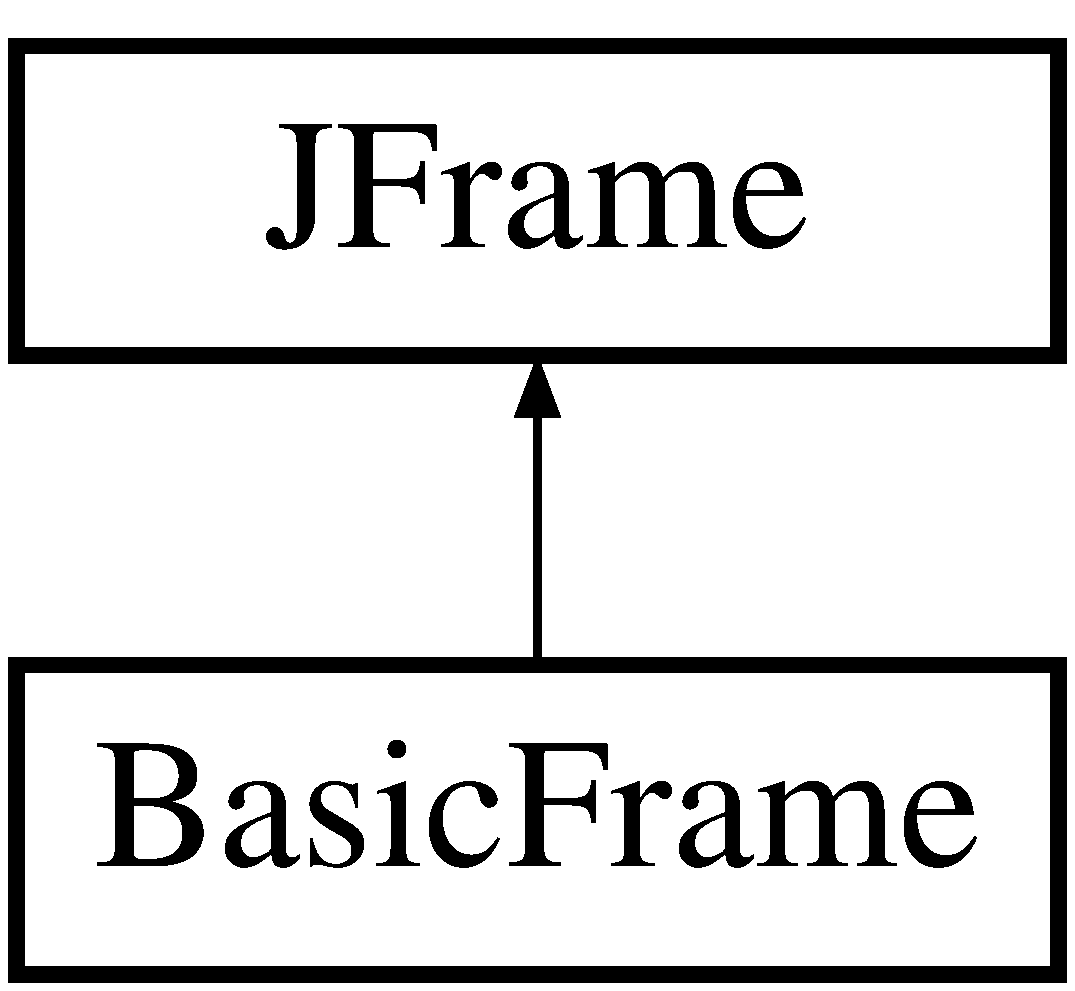
\includegraphics[height=2.000000cm]{class_basic_frame}
\end{center}
\end{figure}
\subsection*{Public Member Functions}
\begin{DoxyCompactItemize}
\item 
{\bf Basic\+Frame} (int type, long init\+Time, long final\+Time, long max\+Time, Array\+List$<$ Array\+List$<$ Long $>$$>$ times)
\begin{DoxyCompactList}\small\item\em \doxyref{Basic\+Frame}{p.}{class_basic_frame} Constructor. \end{DoxyCompactList}\end{DoxyCompactItemize}


\subsection{Detailed Description}
Creates a J\+Frame object to build the main windows for the Graphics  public. 

Definition at line 14 of file Basic\+Frame.\+java.



\subsection{Constructor \& Destructor Documentation}
\index{Basic\+Frame@{Basic\+Frame}!Basic\+Frame@{Basic\+Frame}}
\index{Basic\+Frame@{Basic\+Frame}!Basic\+Frame@{Basic\+Frame}}
\subsubsection[{Basic\+Frame(int type, long init\+Time, long final\+Time, long max\+Time, Array\+List$<$ Array\+List$<$ Long $>$$>$ times)}]{\setlength{\rightskip}{0pt plus 5cm}Basic\+Frame.\+Basic\+Frame (
\begin{DoxyParamCaption}
\item[{int}]{type, }
\item[{long}]{init\+Time, }
\item[{long}]{final\+Time, }
\item[{long}]{max\+Time, }
\item[{Array\+List$<$ Array\+List$<$ Long $>$$>$}]{times}
\end{DoxyParamCaption}
)}\label{class_basic_frame_aeba0120c57b6855a4cd9ba2a8b421018}


\doxyref{Basic\+Frame}{p.}{class_basic_frame} Constructor. 


\begin{DoxyParams}{Parameters}
{\em type,init\+Time,final\+Time,max\+Time,times} & public \\
\hline
\end{DoxyParams}
Makes a layout with x rows but 1 col

Set the layout to the J\+Frame object

Configuration of the window

Adjust dimension

Set main windows location and allow user to finish the execution by closing the window

Creates Panel object, the amount of panels it�s equal to the Array\+List size

Creates a default panel to show general information about the Threads 

Definition at line 22 of file Basic\+Frame.\+java.



The documentation for this class was generated from the following file\+:\begin{DoxyCompactItemize}
\item 
src/{\bf Basic\+Frame.\+java}\end{DoxyCompactItemize}

\section{main Class Reference}
\label{classmain}\index{main@{main}}
\subsection*{Static Public Member Functions}
\begin{DoxyCompactItemize}
\item 
static void {\bf main} (String[$\,$] args)  throws Exception 
\begin{DoxyCompactList}\small\item\em Method Main of the project, where other programs are initialized. \end{DoxyCompactList}\end{DoxyCompactItemize}


\subsection{Constructor \& Destructor Documentation}
\index{main@{main}!main@{main}}
\index{main@{main}!main@{main}}
\subsubsection[{main(\+String[] args)}]{\setlength{\rightskip}{0pt plus 5cm}static void main.\+main (
\begin{DoxyParamCaption}
\item[{String[$\,$]}]{args}
\end{DoxyParamCaption}
) throws Exception\hspace{0.3cm}{\ttfamily [static]}}\label{classmain_a0877f3b412d48b8c92fa25c4b98c2f5a}


Method Main of the project, where other programs are initialized. 


\begin{DoxyParams}{Parameters}
{\em args} & \\
\hline
\end{DoxyParams}

\begin{DoxyExceptions}{Exceptions}
{\em Exception} & \\
\hline
\end{DoxyExceptions}
\begin{DoxyReturn}{Returns}
void  public static 
\end{DoxyReturn}


The documentation for this class was generated from the following file\+:\begin{DoxyCompactItemize}
\item 
src/{\bf main.\+java}\end{DoxyCompactItemize}

\section{Thread\+Panel Class Reference}
\label{class_thread_panel}\index{Thread\+Panel@{Thread\+Panel}}


Creates a J\+Panel object  public.  


Inheritance diagram for Thread\+Panel\+:\begin{figure}[H]
\begin{center}
\leavevmode
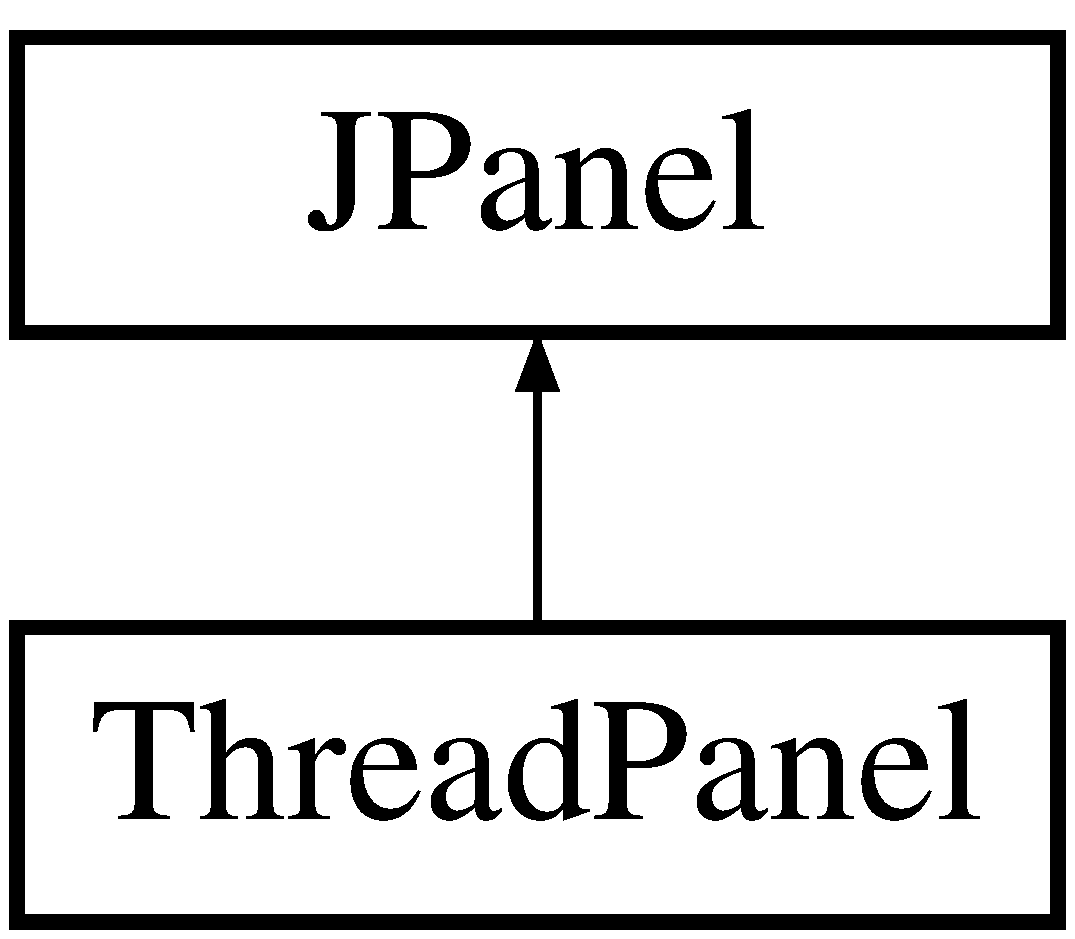
\includegraphics[height=2.000000cm]{class_thread_panel}
\end{center}
\end{figure}
\subsection*{Public Member Functions}
\begin{DoxyCompactItemize}
\item 
{\bf Thread\+Panel} (int id, long init, long end, long max, Array\+List$<$ Array\+List$<$ Long $>$$>$ times)
\begin{DoxyCompactList}\small\item\em \doxyref{Thread\+Panel}{p.}{class_thread_panel} Constructor. \end{DoxyCompactList}\item 
void {\bf paint\+Component} (Graphics g)
\begin{DoxyCompactList}\small\item\em void paint\+Component. Creates the Graphic components on the Frame object \end{DoxyCompactList}\end{DoxyCompactItemize}


\subsection{Detailed Description}
Creates a J\+Panel object  public. 

Definition at line 15 of file Thread\+Panel.\+java.



\subsection{Constructor \& Destructor Documentation}
\index{Thread\+Panel@{Thread\+Panel}!Thread\+Panel@{Thread\+Panel}}
\index{Thread\+Panel@{Thread\+Panel}!Thread\+Panel@{Thread\+Panel}}
\subsubsection[{Thread\+Panel(int id, long init, long end, long max, Array\+List$<$ Array\+List$<$ Long $>$$>$ times)}]{\setlength{\rightskip}{0pt plus 5cm}Thread\+Panel.\+Thread\+Panel (
\begin{DoxyParamCaption}
\item[{int}]{id, }
\item[{long}]{init, }
\item[{long}]{end, }
\item[{long}]{max, }
\item[{Array\+List$<$ Array\+List$<$ Long $>$$>$}]{times}
\end{DoxyParamCaption}
)}\label{class_thread_panel_ac1b6921c24276c643a566e06b87b7d4c}


\doxyref{Thread\+Panel}{p.}{class_thread_panel} Constructor. 


\begin{DoxyParams}{Parameters}
{\em id,init,end,max,times} & public \\
\hline
\end{DoxyParams}


Definition at line 30 of file Thread\+Panel.\+java.



\subsection{Member Function Documentation}
\index{Thread\+Panel@{Thread\+Panel}!paint\+Component@{paint\+Component}}
\index{paint\+Component@{paint\+Component}!Thread\+Panel@{Thread\+Panel}}
\subsubsection[{paint\+Component(\+Graphics g)}]{\setlength{\rightskip}{0pt plus 5cm}void Thread\+Panel.\+paint\+Component (
\begin{DoxyParamCaption}
\item[{Graphics}]{g}
\end{DoxyParamCaption}
)}\label{class_thread_panel_abb56e5001767700781bd6f4984738781}


void paint\+Component. Creates the Graphic components on the Frame object 


\begin{DoxyParams}{Parameters}
{\em g} & \\
\hline
\end{DoxyParams}
\begin{DoxyReturn}{Returns}
void  public 
\end{DoxyReturn}
Shows the Default panel information

Shows the panel information and builds the graphic components

Get the Thread time information

Builds a graphic string on the panel

Draws the x-\/axis line on each panel

Draws the x-\/axis values on each panel

Creates the first point on the x-\/axis

Creates the second point on the x-\/axis

Unification of first and second point on the x-\/axis 

Definition at line 45 of file Thread\+Panel.\+java.



The documentation for this class was generated from the following file\+:\begin{DoxyCompactItemize}
\item 
src/{\bf Thread\+Panel.\+java}\end{DoxyCompactItemize}

\section{With\+Runnable1\+\_\+2 Class Reference}
\label{class_with_runnable1__2}\index{With\+Runnable1\+\_\+2@{With\+Runnable1\+\_\+2}}


A thread is created using the Runnable interface  public.  


Inheritance diagram for With\+Runnable1\+\_\+2\+:\begin{figure}[H]
\begin{center}
\leavevmode
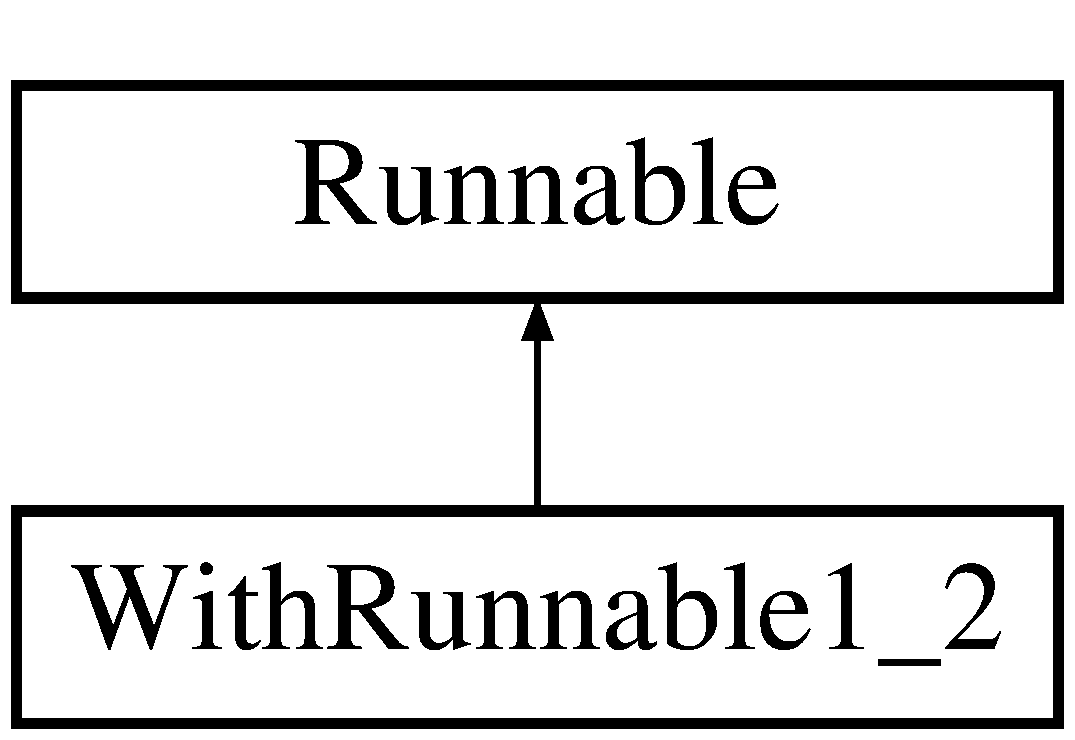
\includegraphics[height=2.000000cm]{class_with_runnable1__2}
\end{center}
\end{figure}
\subsection*{Public Member Functions}
\begin{DoxyCompactItemize}
\item 
void {\bf run} ()
\end{DoxyCompactItemize}


\subsection{Detailed Description}
A thread is created using the Runnable interface  public. 

Definition at line 7 of file With\+Runnable1\+\_\+2.\+java.



\subsection{Member Function Documentation}
\index{With\+Runnable1\+\_\+2@{With\+Runnable1\+\_\+2}!run@{run}}
\index{run@{run}!With\+Runnable1\+\_\+2@{With\+Runnable1\+\_\+2}}
\subsubsection[{run()}]{\setlength{\rightskip}{0pt plus 5cm}void With\+Runnable1\+\_\+2.\+run (
\begin{DoxyParamCaption}
{}
\end{DoxyParamCaption}
)}\label{class_with_runnable1__2_aabb7116851a8c69678945a7953319603}
Run function. Running to start the thread, and displays a message on screen \begin{DoxyReturn}{Returns}
void  public 
\end{DoxyReturn}


Definition at line 15 of file With\+Runnable1\+\_\+2.\+java.



The documentation for this class was generated from the following file\+:\begin{DoxyCompactItemize}
\item 
src/{\bf With\+Runnable1\+\_\+2.\+java}\end{DoxyCompactItemize}

\section{With\+Runnable1\+\_\+3 Class Reference}
\label{class_with_runnable1__3}\index{With\+Runnable1\+\_\+3@{With\+Runnable1\+\_\+3}}


A thread is created using the Runnable interface  public.  


Inheritance diagram for With\+Runnable1\+\_\+3\+:\begin{figure}[H]
\begin{center}
\leavevmode
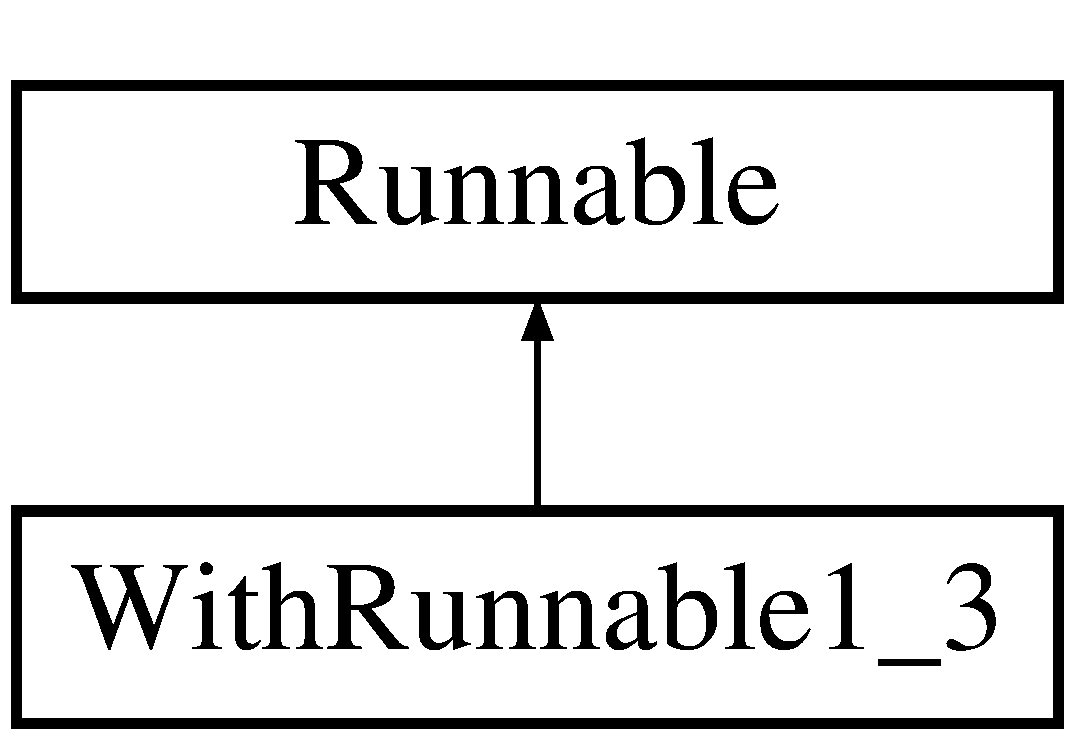
\includegraphics[height=2.000000cm]{class_with_runnable1__3}
\end{center}
\end{figure}
\subsection*{Public Member Functions}
\begin{DoxyCompactItemize}
\item 
void {\bf run} ()
\end{DoxyCompactItemize}


\subsection{Detailed Description}
A thread is created using the Runnable interface  public. 

Definition at line 7 of file With\+Runnable1\+\_\+3.\+java.



\subsection{Member Function Documentation}
\index{With\+Runnable1\+\_\+3@{With\+Runnable1\+\_\+3}!run@{run}}
\index{run@{run}!With\+Runnable1\+\_\+3@{With\+Runnable1\+\_\+3}}
\subsubsection[{run()}]{\setlength{\rightskip}{0pt plus 5cm}void With\+Runnable1\+\_\+3.\+run (
\begin{DoxyParamCaption}
{}
\end{DoxyParamCaption}
)}\label{class_with_runnable1__3_ad8d2bbcfbf2bc20801536854a14abb9b}
Run function. Running to start the thread, and displays a message on screen after one second \begin{DoxyReturn}{Returns}
void  public 
\end{DoxyReturn}


Definition at line 15 of file With\+Runnable1\+\_\+3.\+java.



The documentation for this class was generated from the following file\+:\begin{DoxyCompactItemize}
\item 
src/{\bf With\+Runnable1\+\_\+3.\+java}\end{DoxyCompactItemize}

\section{With\+Runnable2\+\_\+1 Class Reference}
\label{class_with_runnable2__1}\index{With\+Runnable2\+\_\+1@{With\+Runnable2\+\_\+1}}


From the command line parameters receive few threads to create, the program will create and execute the indicated number of threads and show a message on the screen.  public.  


Inheritance diagram for With\+Runnable2\+\_\+1\+:\begin{figure}[H]
\begin{center}
\leavevmode
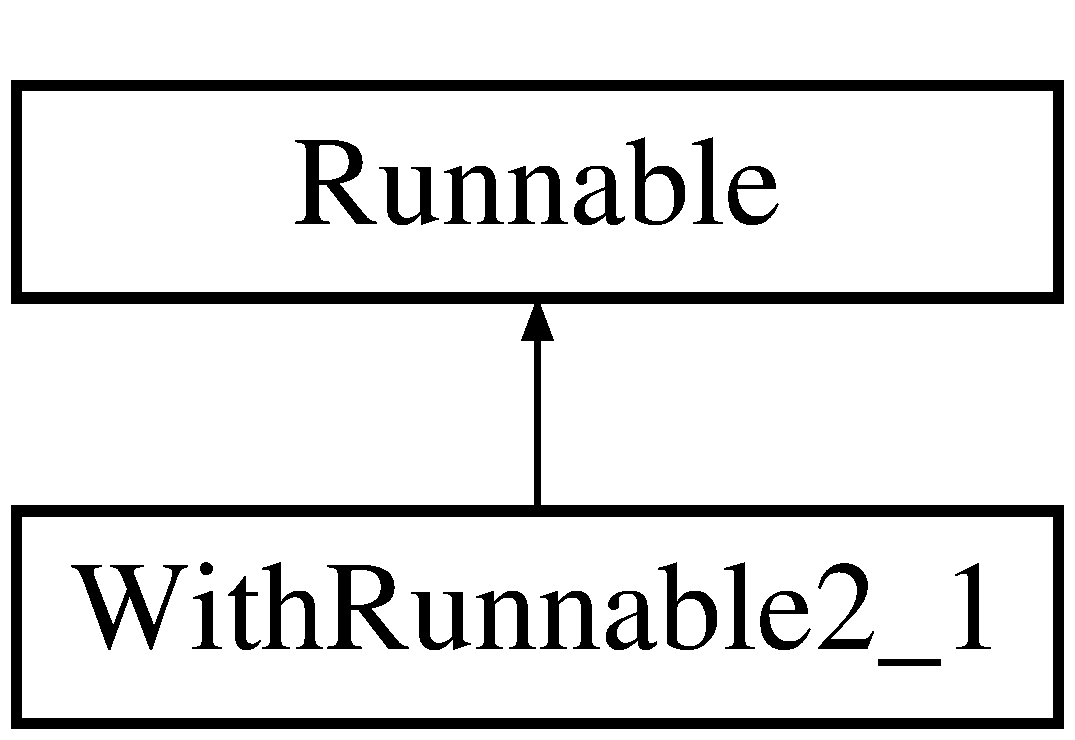
\includegraphics[height=2.000000cm]{class_with_runnable2__1}
\end{center}
\end{figure}
\subsection*{Public Member Functions}
\begin{DoxyCompactItemize}
\item 
{\bf With\+Runnable2\+\_\+1} ()
\begin{DoxyCompactList}\small\item\em \doxyref{With\+Runnable2\+\_\+1}{p.}{class_with_runnable2__1} Constructor  public. \end{DoxyCompactList}\item 
synchronized void {\bf run} ()
\end{DoxyCompactItemize}


\subsection{Detailed Description}
From the command line parameters receive few threads to create, the program will create and execute the indicated number of threads and show a message on the screen.  public. 

Definition at line 7 of file With\+Runnable2\+\_\+1.\+java.



\subsection{Constructor \& Destructor Documentation}
\index{With\+Runnable2\+\_\+1@{With\+Runnable2\+\_\+1}!With\+Runnable2\+\_\+1@{With\+Runnable2\+\_\+1}}
\index{With\+Runnable2\+\_\+1@{With\+Runnable2\+\_\+1}!With\+Runnable2\+\_\+1@{With\+Runnable2\+\_\+1}}
\subsubsection[{With\+Runnable2\+\_\+1()}]{\setlength{\rightskip}{0pt plus 5cm}With\+Runnable2\+\_\+1.\+With\+Runnable2\+\_\+1 (
\begin{DoxyParamCaption}
{}
\end{DoxyParamCaption}
)}\label{class_with_runnable2__1_a1cd16dd9e679245b2741ee453d200926}


\doxyref{With\+Runnable2\+\_\+1}{p.}{class_with_runnable2__1} Constructor  public. 



Definition at line 15 of file With\+Runnable2\+\_\+1.\+java.



\subsection{Member Function Documentation}
\index{With\+Runnable2\+\_\+1@{With\+Runnable2\+\_\+1}!run@{run}}
\index{run@{run}!With\+Runnable2\+\_\+1@{With\+Runnable2\+\_\+1}}
\subsubsection[{run()}]{\setlength{\rightskip}{0pt plus 5cm}synchronized void With\+Runnable2\+\_\+1.\+run (
\begin{DoxyParamCaption}
{}
\end{DoxyParamCaption}
)}\label{class_with_runnable2__1_a7479a6566832e958e8d4015eb7cc60fd}
Synchronized run function. Running to synchronized start the thread, and displays a message on screen, after one second displays other message \begin{DoxyReturn}{Returns}
void  public 
\end{DoxyReturn}


Definition at line 25 of file With\+Runnable2\+\_\+1.\+java.



The documentation for this class was generated from the following file\+:\begin{DoxyCompactItemize}
\item 
src/{\bf With\+Runnable2\+\_\+1.\+java}\end{DoxyCompactItemize}

\section{With\+Runnable2\+\_\+2 Class Reference}
\label{class_with_runnable2__2}\index{With\+Runnable2\+\_\+2@{With\+Runnable2\+\_\+2}}


From the command line parameters receive few threads to create, the program will create and execute the indicated number of threads and show a runtime each thread on the screen.  public.  


Inheritance diagram for With\+Runnable2\+\_\+2\+:\begin{figure}[H]
\begin{center}
\leavevmode
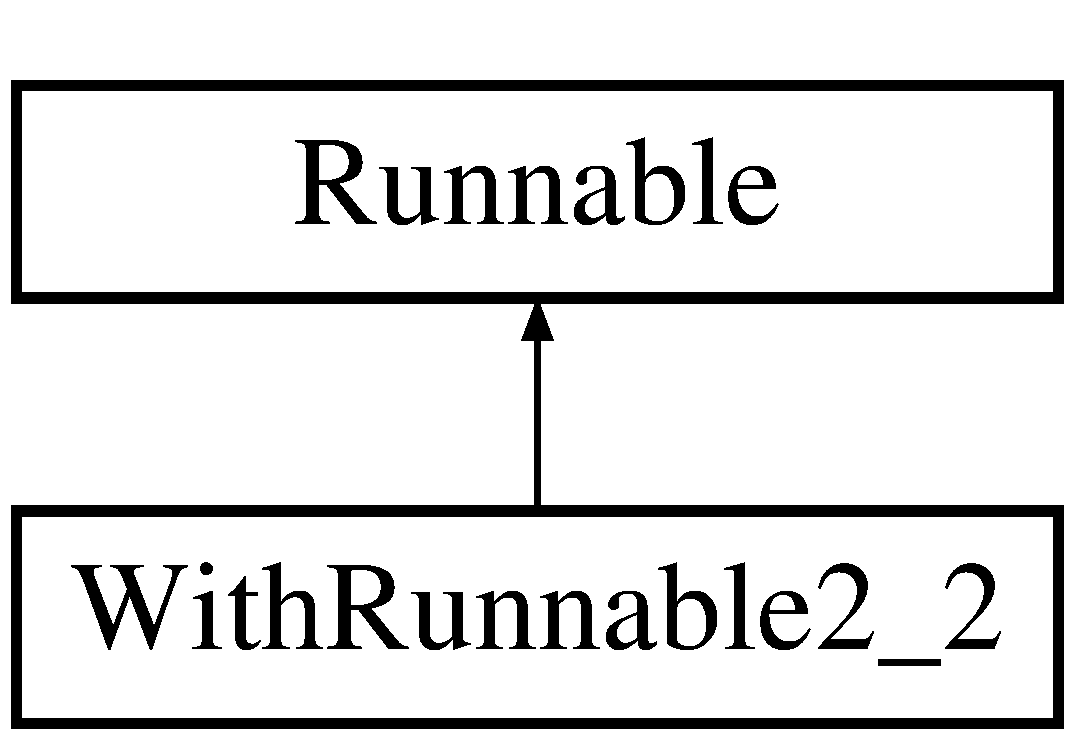
\includegraphics[height=2.000000cm]{class_with_runnable2__2}
\end{center}
\end{figure}
\subsection*{Public Member Functions}
\begin{DoxyCompactItemize}
\item 
{\bf With\+Runnable2\+\_\+2} ()
\begin{DoxyCompactList}\small\item\em \doxyref{With\+Runnable2\+\_\+2}{p.}{class_with_runnable2__2} Constructor  public. \end{DoxyCompactList}\item 
synchronized void {\bf run} ()
\end{DoxyCompactItemize}


\subsection{Detailed Description}
From the command line parameters receive few threads to create, the program will create and execute the indicated number of threads and show a runtime each thread on the screen.  public. 

Definition at line 7 of file With\+Runnable2\+\_\+2.\+java.



\subsection{Constructor \& Destructor Documentation}
\index{With\+Runnable2\+\_\+2@{With\+Runnable2\+\_\+2}!With\+Runnable2\+\_\+2@{With\+Runnable2\+\_\+2}}
\index{With\+Runnable2\+\_\+2@{With\+Runnable2\+\_\+2}!With\+Runnable2\+\_\+2@{With\+Runnable2\+\_\+2}}
\subsubsection[{With\+Runnable2\+\_\+2()}]{\setlength{\rightskip}{0pt plus 5cm}With\+Runnable2\+\_\+2.\+With\+Runnable2\+\_\+2 (
\begin{DoxyParamCaption}
{}
\end{DoxyParamCaption}
)}\label{class_with_runnable2__2_ae6619e279b12305889780366cb2e0b15}


\doxyref{With\+Runnable2\+\_\+2}{p.}{class_with_runnable2__2} Constructor  public. 



Definition at line 15 of file With\+Runnable2\+\_\+2.\+java.



\subsection{Member Function Documentation}
\index{With\+Runnable2\+\_\+2@{With\+Runnable2\+\_\+2}!run@{run}}
\index{run@{run}!With\+Runnable2\+\_\+2@{With\+Runnable2\+\_\+2}}
\subsubsection[{run()}]{\setlength{\rightskip}{0pt plus 5cm}synchronized void With\+Runnable2\+\_\+2.\+run (
\begin{DoxyParamCaption}
{}
\end{DoxyParamCaption}
)}\label{class_with_runnable2__2_a85cab9806b4357d9d3c45c46b7e9551b}
Synchronized run function. Running to synchronized start the thread, and displays a message on screen, after show a runtime each thread \begin{DoxyReturn}{Returns}
void  public 
\end{DoxyReturn}


Definition at line 25 of file With\+Runnable2\+\_\+2.\+java.



The documentation for this class was generated from the following file\+:\begin{DoxyCompactItemize}
\item 
src/{\bf With\+Runnable2\+\_\+2.\+java}\end{DoxyCompactItemize}

\section{With\+Runnable2\+\_\+4 Class Reference}
\label{class_with_runnable2__4}\index{With\+Runnable2\+\_\+4@{With\+Runnable2\+\_\+4}}


From the command line parameters receive few threads to create, the program will create and execute the indicated number of threads and displays the total time it takes to run all the threads on the screen.  public.  


Inheritance diagram for With\+Runnable2\+\_\+4\+:\begin{figure}[H]
\begin{center}
\leavevmode
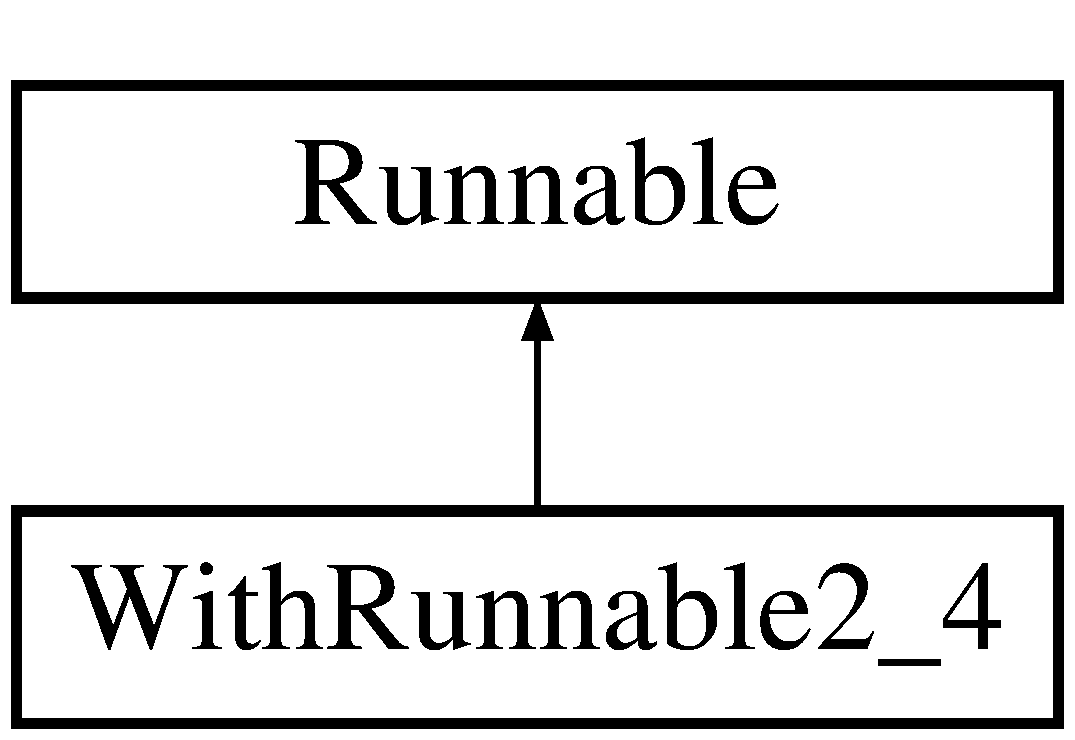
\includegraphics[height=2.000000cm]{class_with_runnable2__4}
\end{center}
\end{figure}
\subsection*{Public Member Functions}
\begin{DoxyCompactItemize}
\item 
{\bf With\+Runnable2\+\_\+4} ()
\begin{DoxyCompactList}\small\item\em \doxyref{With\+Runnable2\+\_\+4}{p.}{class_with_runnable2__4} Constructor  public. \end{DoxyCompactList}\item 
void {\bf set\+Time} (long time)
\begin{DoxyCompactList}\small\item\em Void set\+Time. Add one time in the Array\+List. \end{DoxyCompactList}\item 
Iterator$<$ Long $>$ {\bf get\+Times} ()
\begin{DoxyCompactList}\small\item\em Method get\+Times. Add one time in the Array\+List. \end{DoxyCompactList}\item 
synchronized void {\bf run} ()
\end{DoxyCompactItemize}


\subsection{Detailed Description}
From the command line parameters receive few threads to create, the program will create and execute the indicated number of threads and displays the total time it takes to run all the threads on the screen.  public. 

Definition at line 10 of file With\+Runnable2\+\_\+4.\+java.



\subsection{Constructor \& Destructor Documentation}
\index{With\+Runnable2\+\_\+4@{With\+Runnable2\+\_\+4}!With\+Runnable2\+\_\+4@{With\+Runnable2\+\_\+4}}
\index{With\+Runnable2\+\_\+4@{With\+Runnable2\+\_\+4}!With\+Runnable2\+\_\+4@{With\+Runnable2\+\_\+4}}
\subsubsection[{With\+Runnable2\+\_\+4()}]{\setlength{\rightskip}{0pt plus 5cm}With\+Runnable2\+\_\+4.\+With\+Runnable2\+\_\+4 (
\begin{DoxyParamCaption}
{}
\end{DoxyParamCaption}
)}\label{class_with_runnable2__4_a440a3bce735796f5af5d7630e8850323}


\doxyref{With\+Runnable2\+\_\+4}{p.}{class_with_runnable2__4} Constructor  public. 



Definition at line 19 of file With\+Runnable2\+\_\+4.\+java.



\subsection{Member Function Documentation}
\index{With\+Runnable2\+\_\+4@{With\+Runnable2\+\_\+4}!get\+Times@{get\+Times}}
\index{get\+Times@{get\+Times}!With\+Runnable2\+\_\+4@{With\+Runnable2\+\_\+4}}
\subsubsection[{get\+Times()}]{\setlength{\rightskip}{0pt plus 5cm}Iterator$<$Long$>$ With\+Runnable2\+\_\+4.\+get\+Times (
\begin{DoxyParamCaption}
{}
\end{DoxyParamCaption}
)}\label{class_with_runnable2__4_ab067373007e990dd4b3f3af3a7b3628e}


Method get\+Times. Add one time in the Array\+List. 

\begin{DoxyReturn}{Returns}
Iterator$<$\+Long$>$  public 
\end{DoxyReturn}


Definition at line 40 of file With\+Runnable2\+\_\+4.\+java.

\index{With\+Runnable2\+\_\+4@{With\+Runnable2\+\_\+4}!run@{run}}
\index{run@{run}!With\+Runnable2\+\_\+4@{With\+Runnable2\+\_\+4}}
\subsubsection[{run()}]{\setlength{\rightskip}{0pt plus 5cm}synchronized void With\+Runnable2\+\_\+4.\+run (
\begin{DoxyParamCaption}
{}
\end{DoxyParamCaption}
)}\label{class_with_runnable2__4_a5c16d8b5bc065f242fca06dbf9d8790b}
Synchronized run function. Running to synchronized start the threads, displays a messages on screen and save the times \begin{DoxyReturn}{Returns}
void  public 
\end{DoxyReturn}


Definition at line 50 of file With\+Runnable2\+\_\+4.\+java.

\index{With\+Runnable2\+\_\+4@{With\+Runnable2\+\_\+4}!set\+Time@{set\+Time}}
\index{set\+Time@{set\+Time}!With\+Runnable2\+\_\+4@{With\+Runnable2\+\_\+4}}
\subsubsection[{set\+Time(long time)}]{\setlength{\rightskip}{0pt plus 5cm}void With\+Runnable2\+\_\+4.\+set\+Time (
\begin{DoxyParamCaption}
\item[{long}]{time}
\end{DoxyParamCaption}
)}\label{class_with_runnable2__4_a80897e31f5471b104585fb01d3d89ac4}


Void set\+Time. Add one time in the Array\+List. 


\begin{DoxyParams}{Parameters}
{\em time} & \\
\hline
\end{DoxyParams}
\begin{DoxyReturn}{Returns}
void  public 
\end{DoxyReturn}


Definition at line 30 of file With\+Runnable2\+\_\+4.\+java.



The documentation for this class was generated from the following file\+:\begin{DoxyCompactItemize}
\item 
src/{\bf With\+Runnable2\+\_\+4.\+java}\end{DoxyCompactItemize}

\section{With\+Runnable2\+\_\+6 Class Reference}
\label{class_with_runnable2__6}\index{With\+Runnable2\+\_\+6@{With\+Runnable2\+\_\+6}}


The program creates and executes a growing number of threads, displaying messages on screen and performing mathematical operations and shows a graph in which the number of threads in relation compared with the runtime  public.  


Inheritance diagram for With\+Runnable2\+\_\+6\+:\begin{figure}[H]
\begin{center}
\leavevmode
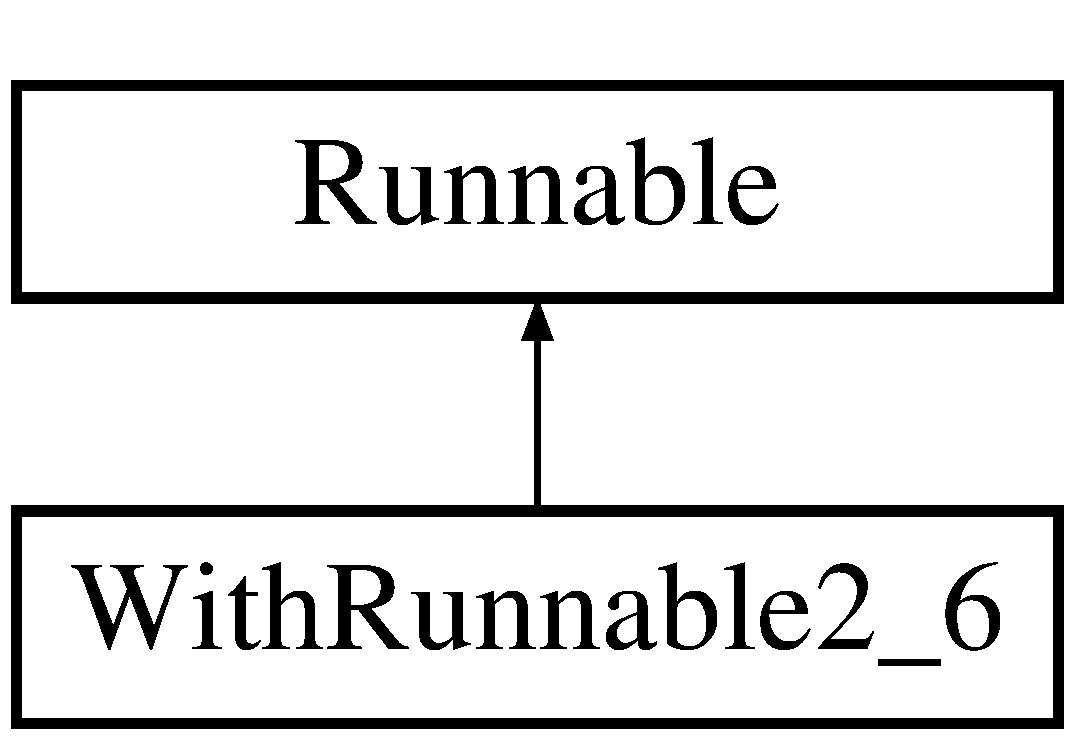
\includegraphics[height=2.000000cm]{class_with_runnable2__6}
\end{center}
\end{figure}
\subsection*{Public Member Functions}
\begin{DoxyCompactItemize}
\item 
{\bf With\+Runnable2\+\_\+6} (int o)
\begin{DoxyCompactList}\small\item\em \doxyref{With\+Runnable2\+\_\+6}{p.}{class_with_runnable2__6} Constructor  public. \end{DoxyCompactList}\item 
void {\bf set\+Init\+Time} (long t)
\begin{DoxyCompactList}\small\item\em void set\+Init\+Time. Saves when the first thread starts the execution \end{DoxyCompactList}\item 
void {\bf set\+Finish\+Time} (long t)
\begin{DoxyCompactList}\small\item\em void set\+Finish\+Time. Saves when the last thread finish the execution \end{DoxyCompactList}\item 
long {\bf get\+Init\+Time} ()
\begin{DoxyCompactList}\small\item\em Method get\+Init\+Time. Get when the last thread starts the execution. \end{DoxyCompactList}\item 
long {\bf get\+Finish\+Time} ()
\begin{DoxyCompactList}\small\item\em Method get\+Finish\+Time. Get when the last thread finish the execution. \end{DoxyCompactList}\item 
Array\+List$<$ Array\+List$<$ Long $>$ $>$ {\bf get\+Times} ()
\begin{DoxyCompactList}\small\item\em Method get\+Times. Get Array\+List of times. \end{DoxyCompactList}\item 
long {\bf get\+Max\+Time} ()
\begin{DoxyCompactList}\small\item\em void add\+Element. Returns the running time of the Threads \end{DoxyCompactList}\item 
synchronized void {\bf run} ()
\end{DoxyCompactItemize}


\subsection{Detailed Description}
The program creates and executes a growing number of threads, displaying messages on screen and performing mathematical operations and shows a graph in which the number of threads in relation compared with the runtime  public. 

Definition at line 10 of file With\+Runnable2\+\_\+6.\+java.



\subsection{Constructor \& Destructor Documentation}
\index{With\+Runnable2\+\_\+6@{With\+Runnable2\+\_\+6}!With\+Runnable2\+\_\+6@{With\+Runnable2\+\_\+6}}
\index{With\+Runnable2\+\_\+6@{With\+Runnable2\+\_\+6}!With\+Runnable2\+\_\+6@{With\+Runnable2\+\_\+6}}
\subsubsection[{With\+Runnable2\+\_\+6(int o)}]{\setlength{\rightskip}{0pt plus 5cm}With\+Runnable2\+\_\+6.\+With\+Runnable2\+\_\+6 (
\begin{DoxyParamCaption}
\item[{int}]{o}
\end{DoxyParamCaption}
)}\label{class_with_runnable2__6_a76e84f507a61504311069733a9de3ce8}


\doxyref{With\+Runnable2\+\_\+6}{p.}{class_with_runnable2__6} Constructor  public. 



Definition at line 29 of file With\+Runnable2\+\_\+6.\+java.



\subsection{Member Function Documentation}
\index{With\+Runnable2\+\_\+6@{With\+Runnable2\+\_\+6}!get\+Finish\+Time@{get\+Finish\+Time}}
\index{get\+Finish\+Time@{get\+Finish\+Time}!With\+Runnable2\+\_\+6@{With\+Runnable2\+\_\+6}}
\subsubsection[{get\+Finish\+Time()}]{\setlength{\rightskip}{0pt plus 5cm}long With\+Runnable2\+\_\+6.\+get\+Finish\+Time (
\begin{DoxyParamCaption}
{}
\end{DoxyParamCaption}
)}\label{class_with_runnable2__6_a5e3ff08cd972f6f814c227e1dbfbd97f}


Method get\+Finish\+Time. Get when the last thread finish the execution. 

\begin{DoxyReturn}{Returns}
long  public 
\end{DoxyReturn}


Definition at line 74 of file With\+Runnable2\+\_\+6.\+java.

\index{With\+Runnable2\+\_\+6@{With\+Runnable2\+\_\+6}!get\+Init\+Time@{get\+Init\+Time}}
\index{get\+Init\+Time@{get\+Init\+Time}!With\+Runnable2\+\_\+6@{With\+Runnable2\+\_\+6}}
\subsubsection[{get\+Init\+Time()}]{\setlength{\rightskip}{0pt plus 5cm}long With\+Runnable2\+\_\+6.\+get\+Init\+Time (
\begin{DoxyParamCaption}
{}
\end{DoxyParamCaption}
)}\label{class_with_runnable2__6_a0abc4f3fc1a30e0dd5e4a96dc136d59e}


Method get\+Init\+Time. Get when the last thread starts the execution. 

\begin{DoxyReturn}{Returns}
long  public 
\end{DoxyReturn}


Definition at line 64 of file With\+Runnable2\+\_\+6.\+java.

\index{With\+Runnable2\+\_\+6@{With\+Runnable2\+\_\+6}!get\+Max\+Time@{get\+Max\+Time}}
\index{get\+Max\+Time@{get\+Max\+Time}!With\+Runnable2\+\_\+6@{With\+Runnable2\+\_\+6}}
\subsubsection[{get\+Max\+Time()}]{\setlength{\rightskip}{0pt plus 5cm}long With\+Runnable2\+\_\+6.\+get\+Max\+Time (
\begin{DoxyParamCaption}
{}
\end{DoxyParamCaption}
)}\label{class_with_runnable2__6_aa3147b9ea15f716263ec7f5faab8cf5a}


void add\+Element. Returns the running time of the Threads 

\begin{DoxyReturn}{Returns}
long  public 
\end{DoxyReturn}


Definition at line 105 of file With\+Runnable2\+\_\+6.\+java.

\index{With\+Runnable2\+\_\+6@{With\+Runnable2\+\_\+6}!get\+Times@{get\+Times}}
\index{get\+Times@{get\+Times}!With\+Runnable2\+\_\+6@{With\+Runnable2\+\_\+6}}
\subsubsection[{get\+Times()}]{\setlength{\rightskip}{0pt plus 5cm}Array\+List$<$Array\+List$<$Long$>$ $>$ With\+Runnable2\+\_\+6.\+get\+Times (
\begin{DoxyParamCaption}
{}
\end{DoxyParamCaption}
)}\label{class_with_runnable2__6_a681715a14a01d8c22c606ba604fd3618}


Method get\+Times. Get Array\+List of times. 

\begin{DoxyReturn}{Returns}
Array\+List$<$Array\+List$<$\+Long$>$$>$  public 
\end{DoxyReturn}


Definition at line 84 of file With\+Runnable2\+\_\+6.\+java.

\index{With\+Runnable2\+\_\+6@{With\+Runnable2\+\_\+6}!run@{run}}
\index{run@{run}!With\+Runnable2\+\_\+6@{With\+Runnable2\+\_\+6}}
\subsubsection[{run()}]{\setlength{\rightskip}{0pt plus 5cm}synchronized void With\+Runnable2\+\_\+6.\+run (
\begin{DoxyParamCaption}
{}
\end{DoxyParamCaption}
)}\label{class_with_runnable2__6_a3a28bdb4607dccf31c1cdbcf1e754d9a}
Synchronized run function. Running to synchronized start the threads, displays a messages on screen and save the times \begin{DoxyReturn}{Returns}
void  public 
\end{DoxyReturn}


Definition at line 161 of file With\+Runnable2\+\_\+6.\+java.

\index{With\+Runnable2\+\_\+6@{With\+Runnable2\+\_\+6}!set\+Finish\+Time@{set\+Finish\+Time}}
\index{set\+Finish\+Time@{set\+Finish\+Time}!With\+Runnable2\+\_\+6@{With\+Runnable2\+\_\+6}}
\subsubsection[{set\+Finish\+Time(long t)}]{\setlength{\rightskip}{0pt plus 5cm}void With\+Runnable2\+\_\+6.\+set\+Finish\+Time (
\begin{DoxyParamCaption}
\item[{long}]{t}
\end{DoxyParamCaption}
)}\label{class_with_runnable2__6_a63c11065e4ae28dd68a3e3e77f80e8b9}


void set\+Finish\+Time. Saves when the last thread finish the execution 


\begin{DoxyParams}{Parameters}
{\em t} & \\
\hline
\end{DoxyParams}
\begin{DoxyReturn}{Returns}
void  public 
\end{DoxyReturn}


Definition at line 54 of file With\+Runnable2\+\_\+6.\+java.

\index{With\+Runnable2\+\_\+6@{With\+Runnable2\+\_\+6}!set\+Init\+Time@{set\+Init\+Time}}
\index{set\+Init\+Time@{set\+Init\+Time}!With\+Runnable2\+\_\+6@{With\+Runnable2\+\_\+6}}
\subsubsection[{set\+Init\+Time(long t)}]{\setlength{\rightskip}{0pt plus 5cm}void With\+Runnable2\+\_\+6.\+set\+Init\+Time (
\begin{DoxyParamCaption}
\item[{long}]{t}
\end{DoxyParamCaption}
)}\label{class_with_runnable2__6_a99fe1b4a2100f69b0edf8f35a1a7a0c2}


void set\+Init\+Time. Saves when the first thread starts the execution 


\begin{DoxyParams}{Parameters}
{\em t} & \\
\hline
\end{DoxyParams}
\begin{DoxyReturn}{Returns}
void  public 
\end{DoxyReturn}


Definition at line 43 of file With\+Runnable2\+\_\+6.\+java.



The documentation for this class was generated from the following file\+:\begin{DoxyCompactItemize}
\item 
src/{\bf With\+Runnable2\+\_\+6.\+java}\end{DoxyCompactItemize}

\section{With\+Runnable3\+\_\+2 Class Reference}
\label{class_with_runnable3__2}\index{With\+Runnable3\+\_\+2@{With\+Runnable3\+\_\+2}}


Case 3.\+2 .The program create and execute the threads and show the difference between the interrupted () and interrupted () methods  public.  


Inheritance diagram for With\+Runnable3\+\_\+2\+:\begin{figure}[H]
\begin{center}
\leavevmode
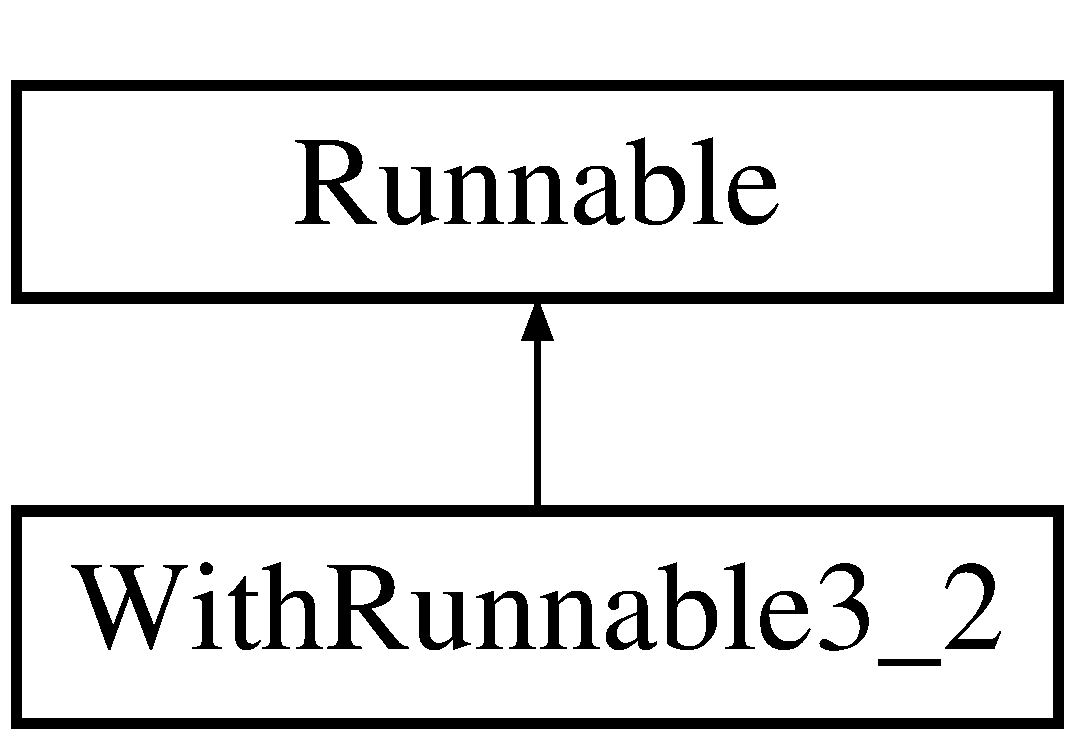
\includegraphics[height=2.000000cm]{class_with_runnable3__2}
\end{center}
\end{figure}
\subsection*{Public Member Functions}
\begin{DoxyCompactItemize}
\item 
{\bf With\+Runnable3\+\_\+2} ()
\begin{DoxyCompactList}\small\item\em \doxyref{With\+Runnable3\+\_\+2}{p.}{class_with_runnable3__2} Constructor  public. \end{DoxyCompactList}\item 
synchronized void {\bf run} ()
\end{DoxyCompactItemize}


\subsection{Detailed Description}
Case 3.\+2 .The program create and execute the threads and show the difference between the interrupted () and interrupted () methods  public. 

Definition at line 8 of file With\+Runnable3\+\_\+2.\+java.



\subsection{Constructor \& Destructor Documentation}
\index{With\+Runnable3\+\_\+2@{With\+Runnable3\+\_\+2}!With\+Runnable3\+\_\+2@{With\+Runnable3\+\_\+2}}
\index{With\+Runnable3\+\_\+2@{With\+Runnable3\+\_\+2}!With\+Runnable3\+\_\+2@{With\+Runnable3\+\_\+2}}
\subsubsection[{With\+Runnable3\+\_\+2()}]{\setlength{\rightskip}{0pt plus 5cm}With\+Runnable3\+\_\+2.\+With\+Runnable3\+\_\+2 (
\begin{DoxyParamCaption}
{}
\end{DoxyParamCaption}
)}\label{class_with_runnable3__2_a7f4a7d09ce712cee3f279dc96a53f408}


\doxyref{With\+Runnable3\+\_\+2}{p.}{class_with_runnable3__2} Constructor  public. 



Definition at line 15 of file With\+Runnable3\+\_\+2.\+java.



\subsection{Member Function Documentation}
\index{With\+Runnable3\+\_\+2@{With\+Runnable3\+\_\+2}!run@{run}}
\index{run@{run}!With\+Runnable3\+\_\+2@{With\+Runnable3\+\_\+2}}
\subsubsection[{run()}]{\setlength{\rightskip}{0pt plus 5cm}synchronized void With\+Runnable3\+\_\+2.\+run (
\begin{DoxyParamCaption}
{}
\end{DoxyParamCaption}
)}\label{class_with_runnable3__2_a723ed10d584339fdaecee9a97aeaa7e6}
Synchronized run function. Running to synchronized start the threads, and displays a message on screen, after five seconds display other message. \begin{DoxyReturn}{Returns}
void  public 
\end{DoxyReturn}


Definition at line 25 of file With\+Runnable3\+\_\+2.\+java.



The documentation for this class was generated from the following file\+:\begin{DoxyCompactItemize}
\item 
src/{\bf With\+Runnable3\+\_\+2.\+java}\end{DoxyCompactItemize}

\section{With\+Runnable3\+\_\+3 Class Reference}
\label{class_with_runnable3__3}\index{With\+Runnable3\+\_\+3@{With\+Runnable3\+\_\+3}}


The program create and execute the thread and and waits for a possible signal to be interrupted by the user.  public.  


Inheritance diagram for With\+Runnable3\+\_\+3\+:\begin{figure}[H]
\begin{center}
\leavevmode
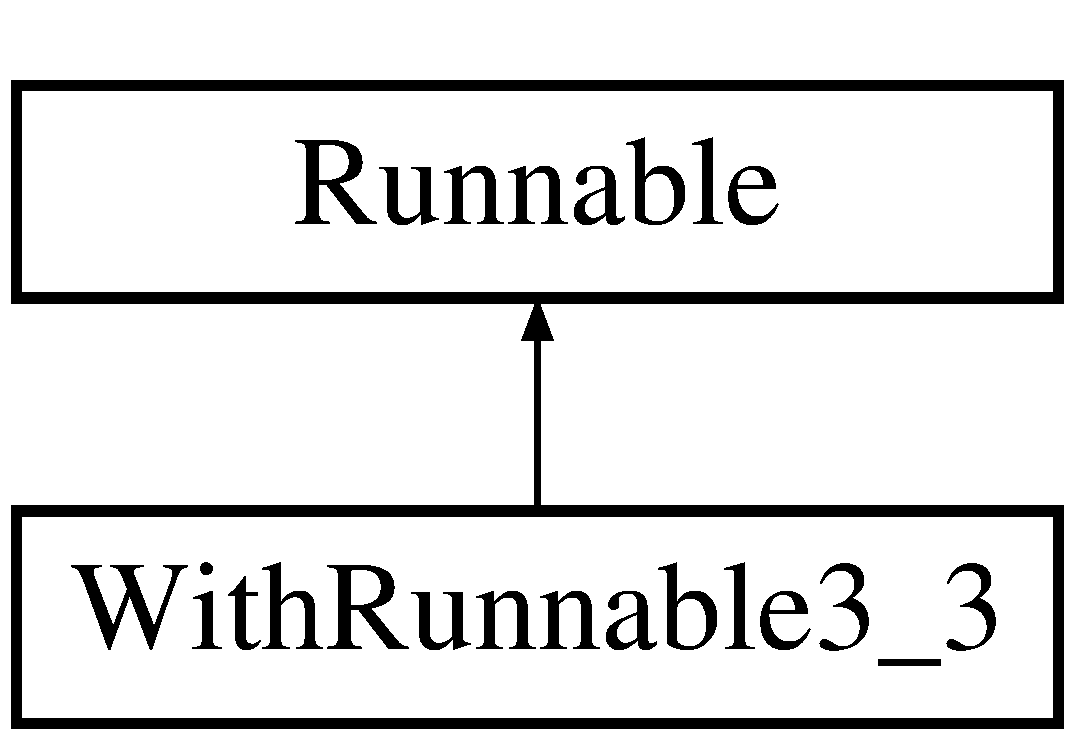
\includegraphics[height=2.000000cm]{class_with_runnable3__3}
\end{center}
\end{figure}
\subsection*{Public Member Functions}
\begin{DoxyCompactItemize}
\item 
void {\bf send\+Signal} ()
\begin{DoxyCompactList}\small\item\em Method send\+Signal. Send a signal for interrupt execution of thread (signal=true) \end{DoxyCompactList}\item 
boolean {\bf get\+Signal} ()
\begin{DoxyCompactList}\small\item\em Method get\+Signal. Observe the state of signal. \end{DoxyCompactList}\item 
void {\bf run} ()
\end{DoxyCompactItemize}


\subsection{Detailed Description}
The program create and execute the thread and and waits for a possible signal to be interrupted by the user.  public. 

Definition at line 7 of file With\+Runnable3\+\_\+3.\+java.



\subsection{Member Function Documentation}
\index{With\+Runnable3\+\_\+3@{With\+Runnable3\+\_\+3}!get\+Signal@{get\+Signal}}
\index{get\+Signal@{get\+Signal}!With\+Runnable3\+\_\+3@{With\+Runnable3\+\_\+3}}
\subsubsection[{get\+Signal()}]{\setlength{\rightskip}{0pt plus 5cm}boolean With\+Runnable3\+\_\+3.\+get\+Signal (
\begin{DoxyParamCaption}
{}
\end{DoxyParamCaption}
)}\label{class_with_runnable3__3_a2892d69fe3a786d4c69642f971d8706d}


Method get\+Signal. Observe the state of signal. 

\begin{DoxyReturn}{Returns}
boolean  public 
\end{DoxyReturn}


Definition at line 26 of file With\+Runnable3\+\_\+3.\+java.

\index{With\+Runnable3\+\_\+3@{With\+Runnable3\+\_\+3}!run@{run}}
\index{run@{run}!With\+Runnable3\+\_\+3@{With\+Runnable3\+\_\+3}}
\subsubsection[{run()}]{\setlength{\rightskip}{0pt plus 5cm}void With\+Runnable3\+\_\+3.\+run (
\begin{DoxyParamCaption}
{}
\end{DoxyParamCaption}
)}\label{class_with_runnable3__3_ab7351a85b08bbe7e3e8be6e112a4f124}
Run function. Running to start the thread, and waits for a possible signal to be interrupted by the user. \begin{DoxyReturn}{Returns}
void  public 
\end{DoxyReturn}


Definition at line 36 of file With\+Runnable3\+\_\+3.\+java.

\index{With\+Runnable3\+\_\+3@{With\+Runnable3\+\_\+3}!send\+Signal@{send\+Signal}}
\index{send\+Signal@{send\+Signal}!With\+Runnable3\+\_\+3@{With\+Runnable3\+\_\+3}}
\subsubsection[{send\+Signal()}]{\setlength{\rightskip}{0pt plus 5cm}void With\+Runnable3\+\_\+3.\+send\+Signal (
\begin{DoxyParamCaption}
{}
\end{DoxyParamCaption}
)}\label{class_with_runnable3__3_a20abc6ac9974a79ed3aac2578ed7754e}


Method send\+Signal. Send a signal for interrupt execution of thread (signal=true) 

\begin{DoxyReturn}{Returns}
void  public 
\end{DoxyReturn}


Definition at line 16 of file With\+Runnable3\+\_\+3.\+java.



The documentation for this class was generated from the following file\+:\begin{DoxyCompactItemize}
\item 
src/{\bf With\+Runnable3\+\_\+3.\+java}\end{DoxyCompactItemize}

\section{With\+Thread1\+\_\+2 Class Reference}
\label{class_with_thread1__2}\index{With\+Thread1\+\_\+2@{With\+Thread1\+\_\+2}}


A thread is created using the Thread class  public.  


Inheritance diagram for With\+Thread1\+\_\+2\+:\begin{figure}[H]
\begin{center}
\leavevmode
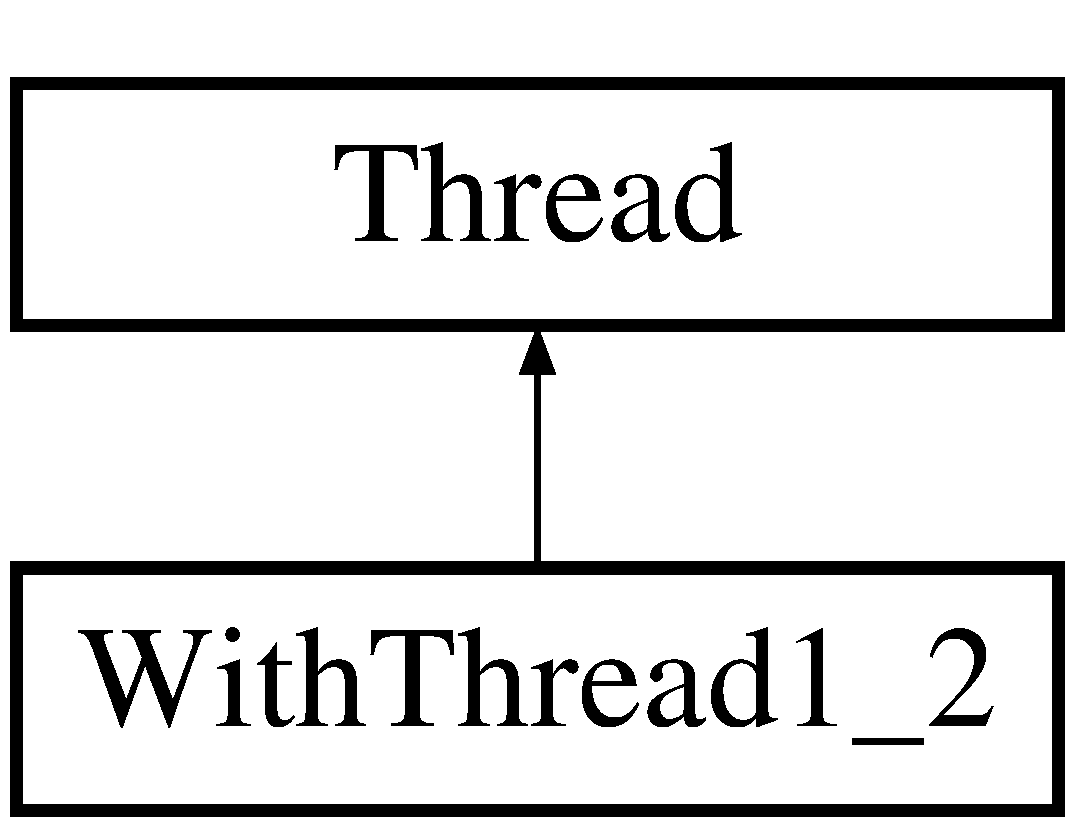
\includegraphics[height=2.000000cm]{class_with_thread1__2}
\end{center}
\end{figure}
\subsection*{Public Member Functions}
\begin{DoxyCompactItemize}
\item 
void {\bf run} ()
\end{DoxyCompactItemize}


\subsection{Detailed Description}
A thread is created using the Thread class  public. 

Definition at line 7 of file With\+Thread1\+\_\+2.\+java.



\subsection{Member Function Documentation}
\index{With\+Thread1\+\_\+2@{With\+Thread1\+\_\+2}!run@{run}}
\index{run@{run}!With\+Thread1\+\_\+2@{With\+Thread1\+\_\+2}}
\subsubsection[{run()}]{\setlength{\rightskip}{0pt plus 5cm}void With\+Thread1\+\_\+2.\+run (
\begin{DoxyParamCaption}
{}
\end{DoxyParamCaption}
)}\label{class_with_thread1__2_a3bbfa1fc716636594b80e68353ee3d63}
Run function. Running to start the thread, and displays a message on screen \begin{DoxyReturn}{Returns}
void  public 
\end{DoxyReturn}


Definition at line 15 of file With\+Thread1\+\_\+2.\+java.



The documentation for this class was generated from the following file\+:\begin{DoxyCompactItemize}
\item 
src/{\bf With\+Thread1\+\_\+2.\+java}\end{DoxyCompactItemize}

\section{With\+Thread1\+\_\+3 Class Reference}
\label{class_with_thread1__3}\index{With\+Thread1\+\_\+3@{With\+Thread1\+\_\+3}}


A thread is created using the Thread class  public.  


Inheritance diagram for With\+Thread1\+\_\+3\+:\begin{figure}[H]
\begin{center}
\leavevmode
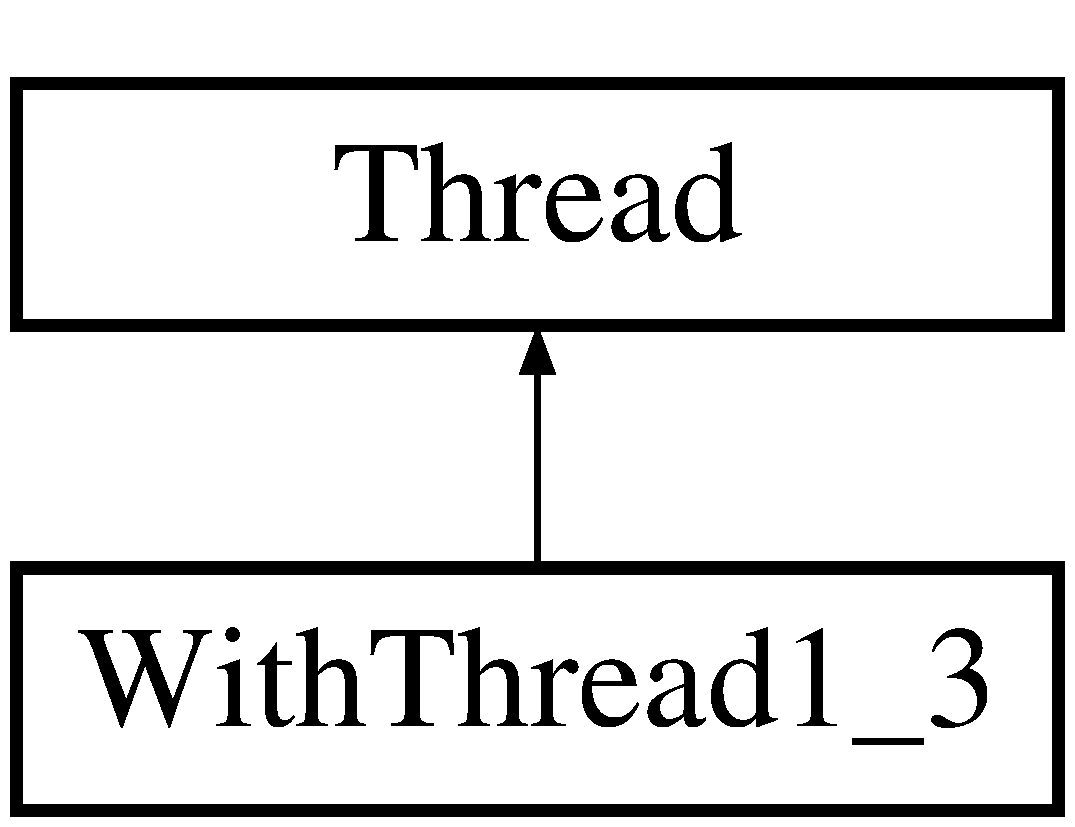
\includegraphics[height=2.000000cm]{class_with_thread1__3}
\end{center}
\end{figure}
\subsection*{Public Member Functions}
\begin{DoxyCompactItemize}
\item 
void {\bf run} ()
\end{DoxyCompactItemize}


\subsection{Detailed Description}
A thread is created using the Thread class  public. 

Definition at line 7 of file With\+Thread1\+\_\+3.\+java.



\subsection{Member Function Documentation}
\index{With\+Thread1\+\_\+3@{With\+Thread1\+\_\+3}!run@{run}}
\index{run@{run}!With\+Thread1\+\_\+3@{With\+Thread1\+\_\+3}}
\subsubsection[{run()}]{\setlength{\rightskip}{0pt plus 5cm}void With\+Thread1\+\_\+3.\+run (
\begin{DoxyParamCaption}
{}
\end{DoxyParamCaption}
)}\label{class_with_thread1__3_a21e941b6dfc037003f1c0f1fa12b3662}
Run function. Running to start the thread, and displays a message on screen after one second \begin{DoxyReturn}{Returns}
void  public 
\end{DoxyReturn}


Definition at line 15 of file With\+Thread1\+\_\+3.\+java.



The documentation for this class was generated from the following file\+:\begin{DoxyCompactItemize}
\item 
src/{\bf With\+Thread1\+\_\+3.\+java}\end{DoxyCompactItemize}

\chapter{File Documentation}
\section{src/\+Basic\+Frame.java File Reference}
\label{_basic_frame_8java}\index{src/\+Basic\+Frame.\+java@{src/\+Basic\+Frame.\+java}}
\subsection*{Classes}
\begin{DoxyCompactItemize}
\item 
class {\bf Basic\+Frame}
\begin{DoxyCompactList}\small\item\em Creates a J\+Frame object to build the main windows for the Graphics  public. \end{DoxyCompactList}\end{DoxyCompactItemize}

\section{C\+:/\+Users/\+Alfredo/workspace/\+P\+\_\+3/src/main.java File Reference}
\label{main_8java}\index{C\+:/\+Users/\+Alfredo/workspace/\+P\+\_\+3/src/main.\+java@{C\+:/\+Users/\+Alfredo/workspace/\+P\+\_\+3/src/main.\+java}}
\subsection*{Classes}
\begin{DoxyCompactItemize}
\item 
class {\bf main}
\end{DoxyCompactItemize}

\section{src/\+Thread\+Panel.java File Reference}
\label{_thread_panel_8java}\index{src/\+Thread\+Panel.\+java@{src/\+Thread\+Panel.\+java}}
\subsection*{Classes}
\begin{DoxyCompactItemize}
\item 
class {\bf Thread\+Panel}
\begin{DoxyCompactList}\small\item\em Creates a J\+Panel object  public. \end{DoxyCompactList}\end{DoxyCompactItemize}

\section{src/\+With\+Runnable1\+\_\+2.java File Reference}
\label{_with_runnable1__2_8java}\index{src/\+With\+Runnable1\+\_\+2.\+java@{src/\+With\+Runnable1\+\_\+2.\+java}}
\subsection*{Classes}
\begin{DoxyCompactItemize}
\item 
class {\bf With\+Runnable1\+\_\+2}
\begin{DoxyCompactList}\small\item\em A thread is created using the Runnable interface  public. \end{DoxyCompactList}\end{DoxyCompactItemize}

\section{src/\+With\+Runnable1\+\_\+3.java File Reference}
\label{_with_runnable1__3_8java}\index{src/\+With\+Runnable1\+\_\+3.\+java@{src/\+With\+Runnable1\+\_\+3.\+java}}
\subsection*{Classes}
\begin{DoxyCompactItemize}
\item 
class {\bf With\+Runnable1\+\_\+3}
\begin{DoxyCompactList}\small\item\em A thread is created using the Runnable interface  public. \end{DoxyCompactList}\end{DoxyCompactItemize}

\section{src/\+With\+Runnable2\+\_\+1.java File Reference}
\label{_with_runnable2__1_8java}\index{src/\+With\+Runnable2\+\_\+1.\+java@{src/\+With\+Runnable2\+\_\+1.\+java}}
\subsection*{Classes}
\begin{DoxyCompactItemize}
\item 
class {\bf With\+Runnable2\+\_\+1}
\begin{DoxyCompactList}\small\item\em From the command line parameters receive few threads to create, the program will create and execute the indicated number of threads and show a message on the screen.  public. \end{DoxyCompactList}\end{DoxyCompactItemize}

\section{src/\+With\+Runnable2\+\_\+2.java File Reference}
\label{_with_runnable2__2_8java}\index{src/\+With\+Runnable2\+\_\+2.\+java@{src/\+With\+Runnable2\+\_\+2.\+java}}
\subsection*{Classes}
\begin{DoxyCompactItemize}
\item 
class {\bf With\+Runnable2\+\_\+2}
\begin{DoxyCompactList}\small\item\em From the command line parameters receive few threads to create, the program will create and execute the indicated number of threads and show a runtime each thread on the screen.  public. \end{DoxyCompactList}\end{DoxyCompactItemize}

\section{src/\+With\+Runnable2\+\_\+4.java File Reference}
\label{_with_runnable2__4_8java}\index{src/\+With\+Runnable2\+\_\+4.\+java@{src/\+With\+Runnable2\+\_\+4.\+java}}
\subsection*{Classes}
\begin{DoxyCompactItemize}
\item 
class {\bf With\+Runnable2\+\_\+4}
\begin{DoxyCompactList}\small\item\em From the command line parameters receive few threads to create, the program will create and execute the indicated number of threads and displays the total time it takes to run all the threads on the screen.  public. \end{DoxyCompactList}\end{DoxyCompactItemize}

\section{src/\+With\+Runnable2\+\_\+6.java File Reference}
\label{_with_runnable2__6_8java}\index{src/\+With\+Runnable2\+\_\+6.\+java@{src/\+With\+Runnable2\+\_\+6.\+java}}
\subsection*{Classes}
\begin{DoxyCompactItemize}
\item 
class {\bf With\+Runnable2\+\_\+6}
\begin{DoxyCompactList}\small\item\em The program creates and executes a growing number of threads, displaying messages on screen and performing mathematical operations and shows a graph in which the number of threads in relation compared with the runtime  public. \end{DoxyCompactList}\end{DoxyCompactItemize}

\section{src/\+With\+Runnable3\+\_\+2.java File Reference}
\label{_with_runnable3__2_8java}\index{src/\+With\+Runnable3\+\_\+2.\+java@{src/\+With\+Runnable3\+\_\+2.\+java}}
\subsection*{Classes}
\begin{DoxyCompactItemize}
\item 
class {\bf With\+Runnable3\+\_\+2}
\begin{DoxyCompactList}\small\item\em Case 3.\+2 .The program create and execute the threads and show the difference between the interrupted () and interrupted () methods  public. \end{DoxyCompactList}\end{DoxyCompactItemize}

\section{src/\+With\+Runnable3\+\_\+3.java File Reference}
\label{_with_runnable3__3_8java}\index{src/\+With\+Runnable3\+\_\+3.\+java@{src/\+With\+Runnable3\+\_\+3.\+java}}
\subsection*{Classes}
\begin{DoxyCompactItemize}
\item 
class {\bf With\+Runnable3\+\_\+3}
\begin{DoxyCompactList}\small\item\em The program create and execute the thread and and waits for a possible signal to be interrupted by the user.  public. \end{DoxyCompactList}\end{DoxyCompactItemize}

\section{src/\+With\+Thread1\+\_\+2.java File Reference}
\label{_with_thread1__2_8java}\index{src/\+With\+Thread1\+\_\+2.\+java@{src/\+With\+Thread1\+\_\+2.\+java}}
\subsection*{Classes}
\begin{DoxyCompactItemize}
\item 
class {\bf With\+Thread1\+\_\+2}
\begin{DoxyCompactList}\small\item\em A thread is created using the Thread class  public. \end{DoxyCompactList}\end{DoxyCompactItemize}

\section{src/\+With\+Thread1\+\_\+3.java File Reference}
\label{_with_thread1__3_8java}\index{src/\+With\+Thread1\+\_\+3.\+java@{src/\+With\+Thread1\+\_\+3.\+java}}
\subsection*{Classes}
\begin{DoxyCompactItemize}
\item 
class {\bf With\+Thread1\+\_\+3}
\begin{DoxyCompactList}\small\item\em A thread is created using the Thread class  public. \end{DoxyCompactList}\end{DoxyCompactItemize}

%--- End generated contents ---

% Index
\backmatter
\newpage
\phantomsection
\clearemptydoublepage
\addcontentsline{toc}{chapter}{Index}
\printindex

\end{document}
